\documentclass[a4paper,11pt]{article}

\usepackage{amsmath, amssymb, amstext, amsfonts, mathrsfs}


% \sffamily %schrift ohne Serifen

\usepackage[T1]{fontenc} 
% schriftencodierung f�r umlaute, trennung
% f\"ur Uni
\usepackage[latin1]{inputenc}
\usepackage{selinput}
% \usepackage[utf8x]{inputenc} 
\usepackage{bibgerm} 
% german bibliography
\usepackage[german]{babel}
%wichtig f�r deutschen Content
\usepackage{ucs}
%erweiterte UTF-8 Unterst�tzung
\usepackage{wrapfig} 
% Paket zur Positionierung einbinden
\usepackage{multirow}
% zusammenfassen von Tabellenzellen
% \usepackage{subscript}
% zum tiefstellen
\usepackage{lscape}
\usepackage{pdflscape}
% zum drehen der Seite
% \usepackage[super]{natbib}
\usepackage[square,sort,comma,numbers]{natbib}
% Erstellung es Literaturverzeichnisses
\usepackage{url}
% Umbruch f�r URL
\usepackage{pst-3dplot}
% f�r tex Grafiken n�tig
\usepackage{pstricks}
\usepackage{listings}
% f�r das einf�gen von Quelltext
\definecolor{codegray}{rgb}{0.92,0.92,0.92}
\lstset{basicstyle=\fontsize{9}{11}\selectfont\ttfamily, breaklines=true, backgroundcolor=\color{codegray}, numbers=left, numberstyle=\tiny, tabsize=4, language=java}
\definecolor{mymauve}{rgb}{0.58,0,0.82}
\definecolor{mygreen}{rgb}{0,0.6,0}
\lstset{
commentstyle=\color{mygreen},
keywordstyle=\color{mymauve},
language=Java,
stringstyle=\color{blue}
}


%Einstellungen f�r Quellcode
\usepackage[a4paper, left=3cm, right=2cm, top=2cm]{geometry}
% Formatierung R�nder
\usepackage[section]{placeins}
% f�r Floatbarriere
\usepackage{color}
\usepackage{colortbl}
%f�r die Verwendung von Farben

\clubpenalty = 10000 
\widowpenalty = 10000
\displaywidowpenalty = 10000
%Verhinderung von Hurenkindern und Schusterjungen
%10000 bedeutet die sie sollen kommplett vermieden werden

\title{Entwicklung einer Android-Applikation f�r die Alarmierung der Einsatzkr�fte der Freiwilligen Feuerwehren}

\author{Sebastian Rieger}

\pagenumbering{arabic}
%Seitenzahlen(arabische Zahlen)

\setlength{\parindent}{0.25cm} 
%Absatzeinzug �ndern in Zoll
\setlength{\parskip}{0.25cm}
%Absatzabstand
\linespread {1.5}
%Zeilenabstand

\usepackage{setspace}
\usepackage{hyperref}
%anklickbare Hyperlinks

%funktioniert nicht bei Fu�noten
\usepackage{graphicx}
\usepackage{graphics}
%f�r einbinden von Grafiken

\usepackage{framed}
%f�r Umrandung der Erkl�rung
\usepackage{acronym}
% f�r abk�rzungen
% \usepackage{PSTricks}
\usepackage{epstopdf}
% f�r eps bilder nutze pdflatex --shell-escape this.tex
\usepackage{amssymb}
% f�r mathematische Symbole

\usepackage{hyperref}
% klickbare links

% \usepackage{pdfpages}
\usepackage{rotating}
\usepackage{svg}
%%%%%%%%%%%%%%%%%%%%%%%%%%%%%%%%%%%%%%%%%%%%%%%%%%%%%%%%%%%%%%%%%%%%%%%%%%%%%%%%%%%%%%%%%%%%%%%%%%%%%
%% Angaben zur Arbeit
%%%%%%%%%%%%%%%%%%%%%%%%%%%%%%%%%%%%%%%%%%%%%%%%%%%%%%%%%%%%%%%%%%%%%%%%%%%%%%%

\newcommand{\Autor}{Sebastian Rieger}
\newcommand{\MatrikelNummer}{10286908}
\newcommand{\Kursbezeichnung}{TINF12B1}

\newcommand{\FirmenName}{PDV Systeme}
\newcommand{\FirmenStadt}{Erfurt}
\newcommand{\FirmenLogoDeckblatt}{{\includegraphics[width=3cm]{}}}

% Falls es kein Firmenlogo gibt:
%  \newcommand{\FirmenLogoDeckblatt}{}

\newcommand{\BetreuerFirma}{Prof. Rolf Kruse}
\newcommand{\BetreuerDHBW}{Prof. Steffen Avemarg}
\newcommand{\Titel}{Entwicklung eines Natural User Interface mit Hilfe moderner AR und AI Technologien}
\newcommand{\AbgabeDatum}{15.11.2017}

\newcommand{\Dauer}{24 Wochen}

% \newcommand{\Abschluss}{Bachelor of Engineering}
\newcommand{\Abschluss}{Master of Science}

\newcommand{\Studiengang}{Angewandte Informatik}
% \newcommand{\Studiengang}{Angewandte Informatik}
\newcommand{\Was}{Masterarbeit}

%%%%%%%%%%%%%%%%%%%%%%%%%%%%%%%%%%%%%%%%%%%%%%%%%%%%%%%%%%%%%%%%%%%%%%%%%%%%%%%%%%%%%%%%%%%%%%%%%%%%% 
%steuervariable
\usepackage{ifthen} %Package f�r if/else
\newboolean{bilder} %Deklaration
\setboolean{bilder}{true} %Zuweisung
% \setboolean{bilder}{false} %Zuweisung
%%%%%%%%%%%%%%%%%%%%%%%%%%%%%%%%%%%%%%%%%%%%%%%%%%%%%%%%%%%%%%%%%%%%%%%%%%%%%%%%%%%%%%%%%%%%%%%%%%%%%

\lstdefinelanguage{JavaScript}{
  keywords={typeof, new, true, false, catch, function, return, null, catch, switch, var, if, in, while, do, else, case, break},
  keywordstyle=\color{blue}\bfseries,
  ndkeywords={class, export, boolean, throw, implements, import, this},
  ndkeywordstyle=\color{darkgray}\bfseries,
  identifierstyle=\color{black},
  sensitive=false,
  comment=[l]{//},
  morecomment=[s]{/*}{*/},
  commentstyle=\color{purple}\ttfamily,
  stringstyle=\color{red}\ttfamily,
  morestring=[b]',
  morestring=[b]"
}


\makeatletter
\newcommand\footnoteref[1]{\protected@xdef\@thefnmark{\ref{#1}}\@footnotemark}
\makeatother

\begin{document}

\begin{center}
\vspace*{-2cm}
\hfill
\includegraphics[width=4cm]{Bilder/logo_FHE}\\[1cm]
{\Huge \Titel}\\[2cm]
{\Huge\scshape \Was}\\[2cm]
% {\large f�r die Pr�fung zum}\\[0.5cm]
% {\Large \Abschluss}\\[0.5cm]
% {\large des Studienganges \Studiengang}\\[0.5cm]
{\large \Studiengang}\\[0.5cm]
{\large an der}\\[0.5cm]
{\large Fachhochschule Erfurt}\\[0.5cm]
{\large von}\\[0.5cm]
{\large\bfseries \Autor}\\[1cm]
{\large Abgabedatum \AbgabeDatum}
\vfill
\end{center}
\begin{tabular}{l@{\hspace{1cm}}l}
Bearbeitungszeitraum             & \Dauer                       \\
Matrikelnummer                   & \MatrikelNummer              \\
% Kurs                             & \Kursbezeichnung             \\
% Ausbildungsfirma                 & \FirmenName                  \\
%                                  & \FirmenStadt                 \\
Betreuer der Masterarbeit    & \BetreuerFirma               \\
Zweitbetreuer der Masterarbeit     & \BetreuerDHBW                \\
\end{tabular}

\newpage
%Seitenumbruch
%%%%%%%%%%%%%%%%%%%%%%%%%%%%%%%%%%%%%%%%%%%%%%%%%%%%%%%%%%%%%%%%%%%%%%%%%%%%%%
%% Descr:       Vorlage für Berichte der DHBW-Karlsruhe, Erklärung
%% Author:      Prof. Dr. Jürgen Vollmer, vollmer@dhbw-karlsruhe.de
%% $Id: erklaerung.tex,v 1.2 2010/07/22 13:30:27 vollmer Exp $
%%%%%%%%%%%%%%%%%%%%%%%%%%%%%%%%%%%%%%%%%%%%%%%%%%%%%%%%%%%%%%%%%%%%%%%%%%%%%%%

% In Bachelorarbeiten muss eine schriftliche Erklärung abgegeben werden. In allen anderen
% Arbeiten entf�llt diese. Hierin best�tigen die Studierenden, dass die Bachelorarbeit
% selbst�ndig verfasst und s�mtliche Quellen und Hilfsmittel angegeben sind. Diese Erkl�rung
% bildet das zweite Blatt der Arbeit. Der Text dieser Erkl�rung muss auf einer separaten Seite
% wie unten angegeben lauten.

\newpage
\thispagestyle{empty}
\begin{framed}
\begin{center}
\Large\bfseries Erkl\"arung
\end{center}

\noindent
Ich, \Autor, versichere hiermit, dass ich die vorliegende Masterarbeit mit dem
Thema
"`\Titel"'
selbstst�ndig und nur unter Verwendung der angegebenen Quellen und Hilfsmittel angefertigt
habe.

\vspace{3cm}
\noindent
\underline{\hspace{4cm}}\hfill\underline{\hspace{6cm}}\\
Ort~~~~~Datum\hfill Unterschrift\hspace{4cm}
\end{framed}

%%%%%%%%%%%%%%%%%%%%%%%%%%%%%%%%%%%%%%%%%%%%%%%%%%%%%%%%%%%%%%%%%%%%%%%%%%%%%%%
\endinput
%%%%%%%%%%%%%%%%%%%%%%%%%%%%%%%%%%%%%%%%%%%%%%%%%%%%%%%%%%%%%%%%%%%%%%%%%%%%%%%

\newpage
\begin{spacing}{0.9}

%Einf�gen Inhaltsverzeichnis
\tableofcontents
\newpage
\section{Abstract}
\newpage
\section{Einleitung}
In den letzten zwanzig Jahren hat sich die Bedienung von Computern grundlegend ge�ndert. Vor nicht all zu vielen Jahren gab es nur die M�glichkeit mit Hilfe von Maus und Tastatur mit einem Computer zu interagieren. 

Mit dem Aufkommen von Touch-Screens jedoch �nderte sich auch die Benutzung von Computern. Es war nun m�glich, direkt mit dem Bildschirm zu interagieren ohne den Umweg �ber die Maus.

Als dann wenig sp�ter die ersten Sprachsteuerungen auf den Markt kamen, �nderte sich die Interaktion mit dem Computer erneut. So ist es nun m�glich, Computern mittels Sprache Befehle zu erteilen oder Texte zu sprechen, welche automatisch transkribiert werden.

Heute ist es mit manchen Smartphones schon m�glich, Nachrichten wie SMS zu schreiben und zu versenden, ohne das Telefon �berhaupt in die Hand zu nehmen. Dies ist nur durch neuste Entwicklungen in der \ac{KI} m�glich.

Im selben Zeitraum hat sich parallel auch die \ac{VR} entwickelt. Sie versucht Menschen mit Hilfe von verschiedenen Brillen in eine virtuelle Welt zu versetzen. Die Entwicklungen solcher \ac{VR} Systeme wurde vor allem von der Spieleindustrie getrieben, da sie immer neue Versuche unternimmt, Spieler besser in die Welt des Spiels zu versetzen. 

Eine Abstufung der \ac{VR} ist die \ac{AR}, welche versucht die analoge, reale Welt um digitale Inhalte zu erweitern. Hierbei sind die M�glichkeiten f�r den Einsatz von \ac{AR} fast unbegrenzt. 
Es ist also quasi m�glich, jede menschliche T�tigkeit durch die \ac{AR} zu unterst�tzen. 

Genau hier setzt der Schwerpunkt der Arbeit an. Im Verlauf soll versucht werden, ein \ac{NUI} unter Zuhilfenahme moderner \ac{AR} und \ac{KI} Technologien zu erstellen.

Hierf�r werden aktuelle \ac{AR} und \ac{KI} Systeme daraufhin untersucht, wie sie im Zusammenspiel ein \ac{NUI} bilden k�nnen, welches allein durch Sprache und Gesten mit einem Computer interagiert.

Es soll eine �bliche T�tigkeit mit Hilfe einer \ac{AR} Technologie in der realen Welt abgebildet werden, welche dann von einem Menschen nur unter Zuhilfenahme von Sprache und Gesten gesteuert und bearbeitet werden kann.
\newpage
\section{Augumented Reality}
\newpage
\section{Artificial Intelligence}
Als \ac{AI} oder im deutschen auch \emph{artifizielle Intelligenz} oder \emph{k�nstliche Intelligenz}, bezeichnet, in der Informatik, ein System welches eine Automatisierte Intelligenz besitzt. Eine eindeutige Definition f�r \ac{AI} gibt es nicht, da es schon in der Psychologie an einer genauen Definition mangelt. \cite{WikiKI}

In der heutigen Zeit werden Systeme und Algorithmen die auf neuronalen Netzen basieren als ann�hernd intelligent bezeichnet. Ein Beispiel hierf�r ist "`Google Translate"' welches zwischen verschiedenen Sprachen mittels neuronalen Netz �bersetzt. \cite{TranslateKI}

Es gibt aber auch intelligente Systeme wie "`IBM Watson"', welche nicht auf neuronalen Netzen basieren und ann�hernd intelligent wirken. Diese Intelligenz ist das Resultat einer sehr gro�en Wissensbasis und verschiedenen kombinatorischen Algorithmen. Um zu zeigen wie Leistungsf�hig Watson ist, trat er 2011 in der Quizshow "`Jeopardy"' an und gewann gegen die weltbesten Spieler. \cite{IBMWatson}

\subsection{Sprachassistenten}

Im allgemeinen Sprachgebrauch werden als \ac{AI} die heute �blichen Sprachassistenten wie Siri, Alexa, Cortana oder Google Assistent bezeichnet. Das im Verlauf der Arbeit zu entwickelnde \ac{NUI} soll auf einen dieser Assistenten aufbauen.

Die Entwicklung einer eigenen Spracherkennung ist im Rahmen dieser Arbeit nicht m�glich, da dies sehr viel Zeit und Arbeit in Anspruch nimmt. Selbst Firmen wie Google oder Amazon ben�tigten mehrere Jahre um ihre Assistent auf das aktuelle Leistungsniveau zu heben.

\subsection{Funktionsweise der Sprachassistenten}
Auch wenn die genauen Implementierungen der Sprachassistenten verschiedenen ist, so haben sie alle eins gemenisam und zwar ist dies der Weg der Sprachverarbeitung.

Die Funktionsweise von Siri udn Co. ist recht einfach gehalten. Der Nutzer l�st mit einem Stichwort, "`Hey, Siri..."', "`Ok, Google..."' (Abbildung \ref{assistent_img} 1.)und so weiter, die Benutzung aus. Der darauf folgende Sprachbefehl wird aufgezeichnet und komprimiert an einen Server weitergeleitet (Abbildung \ref{assistent_img} 2.), welcher den gesprochenen Text auswertet und in schriftliche Befehle umwandelt (Abbildung \ref{assistent_img} 3.). Diese Befehle werden dann umgehend zur�ck an das Endger�t des Nutzers Versand (Abbildung \ref{assistent_img} 4.), welches nun auf die Befehle reagieren kann (Abbildung \ref{assistent_img} 5.). In Abbildung \ref{assistent_img} ist dieses vorgehen noch einmal schematisch Dargestellt. \cite{AIGrundlagen}

?????\textcolor{red}{ Wie sieht es besser aus? Verweis auf Abb. oder einzelnen Punkte angeben? oder punkte ganz weglassen? }?????

\begin{figure}[!ht]
\centering
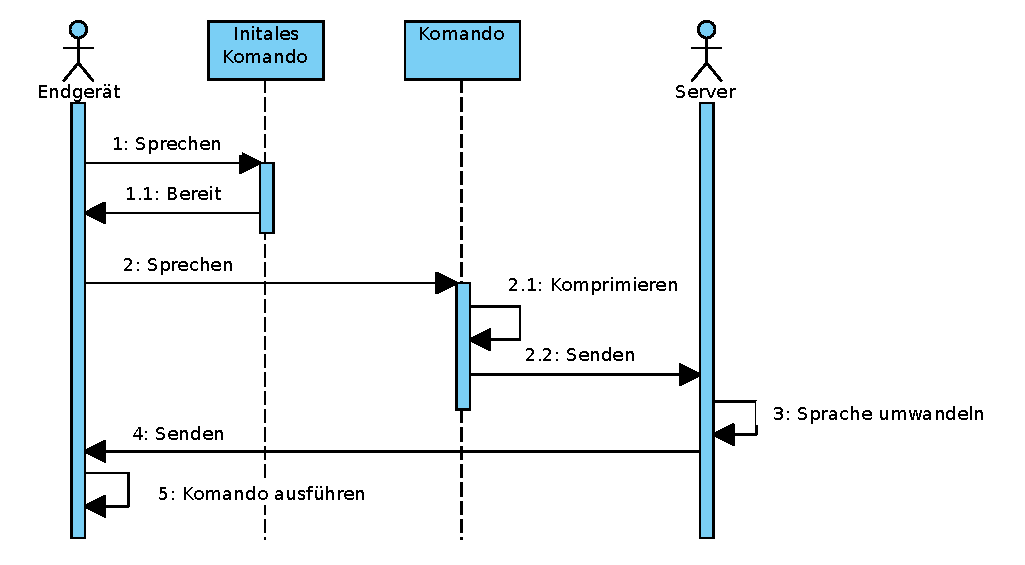
\includegraphics[width=14cm]{Bilder/Assistenten.eps}
\caption{Schematische Darstellung der Kommunikation von Sprachassistenten}
\label{assistent_img}
\centering
\end{figure}

\FloatBarrier

Hierbei ist zu beachten, dass jegliche Kommunikation zwischen Endger�t und Server bei allen Assistenten �ber HTTPS gesichert ist.

Innerhalb der Server, welche die Sprache zu Text wandeln, kommen fast immer neuronale Netze zum einsatz, da nur sie in der Lage sind schnell und eindeutig die Spachbefehle zu wandeln.
Durch die geh�ufte Verwendung mit immer neuen Stimmen und Befehlen lernen die Systeme immer mehr hinzu und k�nnen so die Anfragen immer schneller und besser umwandeln. Dies hat zur Folge, das ein System besser wird, je h�ufiger es genutzt wird.

In den nun folgenden Abschnitten werden die genannten Assistenten auf ihre M�glichkeiten untersucht.

\subsection{Untersuchung der Sprachassistenten}
Es soll nun untersucht werden, in wie weit die heute g�ngigen Assistenten genutzt werden k�nnen, um eine Sprachsteuerung f�r ein \ac{NUI} (siehe Kapitel ?????) umzusetzen.

Hierbei muss der Assistent folgende Kriterien erf�llen:
\begin{itemize}
 \item Lauff�gig auf der Microsoft HoloLens
 \item Offene Programmierschnittstelle (\ac{SDK})
 \item M�glichkeit eigener Sprachkomandos
\end{itemize}

\subsubsection{Siri}
Der wohl �lteste und bekannteste Sprachassistent ist "`Siri"'. Siri ist eine Software zur Spracherkennung und wurde von Apple im Jahre 2010 zusammen mit der Firma Siri Inc. von Apple aufgekauft. Schon ein Jahr sp�ter wurde der Assistent im Zuge der Ver�ffentlichung des iPhone 4s vorgestellt und ver�ffentlicht.

Siri ist eine propriet�re Software und nur iOS, machOS, watchOS und tvOS einsetzbar, weshalb eine Verwendung auf der HoloLens nicht m�glich ist. Zwar verf�gt Siri �ber ein offenes \ac{SDK}, dieses ist jedoch nur f�r Apple eigene Betriebssysteme ausgelegt. \cite{SiriKit} \cite{SiriKit2}


\subsubsection{Alexa}
Alexa ist der Name des Sprachassistenten, welcher von Amazon entwickelt wird und im November 2014 ver�ffentlicht wurde. Seither entwickelt Amazon seinen digitalen Assistenten stetig weiter. 
\cite{WikiAlexa}

Grunds�tzlich funktioniert auch Alexa wie schon im Abschnitt ????? beschrieben. Alexa arbeitet mit sogenannten Skills. Diese erm�glichen es Entwicklern den Assistent mit neuen Funktionen zu erweitern. Will ein Nutzer diesen Skill verwenden, muss er ihn zun�chst innerhalb seines pers�nlichen Assistenten installieren. Danach beherrscht Alexa die entsprechenden Kommandos des Skills. \cite{AmzSkills}

Die eigentlichen Skills, also kleine Programme, welche innerhalb der Amazon Cloud ausgef�hrt und durch den Assistenten gestartet werden k�nnen entweder in Java oder Node.js geschrieben werden. Um diese sp�ter zu ver�ffentlichen muss der Entwickler �ber ein Amazon Developer Account verf�gen.

Amazon verfolgt zur Zeit eine gro�e Marketing-Offensive, welche f�r verschiedene Produkte der Amazon Echo Serie, welche Alexa integriert haben.
Zus�tzlich ist es m�glich Alexa auch auf eigenen Ger�ten verf�gbar zu machen. Hierf�r wird das \ac{AVS} ben�tigt. Dieses \ac{SDK} erm�glicht es den Amazon Assistent auch auf Ger�ten verf�gbar zu machen, welche nicht von Amazon hergestellt wurden. \cite{AVS}

Mit den Skills und dem \ac{AVS}-\ac{SDK}, welches C++ basiert ist, ist es m�gliche alle Ger�te die ein Mikrofon besitzen mit dem Amazon Assistenten auszustatten.

Ein weiterer Vorteil von Alexa sind die sogenannten Speechcons. Diese werden speziell von Amazon zur Verf�gung gestellt, um eine m�glichst nat�rliche und vor allem richtig betonte Aussprache zu gew�hrleisten. Speechcons sind kurze Phrasen, welche in der Regel Umgangssprachlich genutzt werden, wie zum Beispiel der Ausspruch "`ich glaub mein Schwein pfeift"' oder "`Pustekuchen"'. Zus�tzlich steht mit "`Whispers"' auch ein Modus bereit, welcher Alexa fl�stern l�sst. \cite{GolemAlexa} \cite{Speechcons} 

All dies, macht Alexa zumindest f�r den Zuh�rer momentan zu den besten Assistenten auf den Markt.

\subsubsection{Cortana}
Nutzer von "`Windows 10"', einer Xbox oder eines Windows Phone kennen sie bereits, "`Cortana"', den digitalen Assistenten, welcher von Microsoft entwickelt wurde.  Er wurde im Jahr 2014 ver�ffentlicht und steht neben den genannten Microsoft Ger�ten auch f�r Android und iOS zur Verf�gung. Grunds�tzlich kann Cortana eine Suche starten, Programme ausf�hren oder Termine und Notizen verwalten. \cite{WikiCortana}

�ber Skills k�nnen Entwickler �hnlich wie bei Alexa zus�tzliche Funktionen erstellen und f�r Nutzer freigeben. Das von Microsoft bereitgestellte Skills Kit ist momentan noch nicht freigegeben und befindet sich aktuell in einer �ffentlichen Beta-Phase.

Skills f�r Cortana werden �hnlich wie die von Alexa in der Clound ausgef�hrt und k�nnen in .NET oder Node.js geschrieben werden. \cite{Cortana}

\subsubsection{Google Assistent}
Der Google Assistant ist ein Assistent, welcher von Google entwickelt wird und 2016 als Nachfolger von Google Now erschienen ist. \cite{GoogleAssistant}

Eine Besonderheit dieses Assistenten ist, das er Fragen auch aus dem Kontext fr�her gestellter Fragen beantworten kann. So kann ein Nutzer zum Beispiel Fragen "`In welchem Verein spielt Manuel Neuer?"'. Wenn als n�chstes die Frage "`Wie alt ist er?"' folgt, kann der Google Assistent aus dem Kontext schie�en, das ebenfalls "`Manuel Neuer"' als "`er"' gemeint ist. \cite{AssistantBild}

Der Google Assistant ist durch eine Vielzahl von \ac{SDK}s wie zum Beispiel Android, Apple, C++, Python und weitere unter quasi allen Plattformen lauff�hig. \cite{ApiAI}

Mit sogenannten "`Agents"' ist es m�glich, �hnlich wie mit Alexa Skills, �ber ein Web-Interface neue Funktionen zu erstellen.

\subsubsection{Auswertung der M�glichkeiten}
Nach dem �berblick �ber die vier Assistenten Siri, Alexa, Cortana und Google Assistent wird nun ausgewertet welcher am besten f�r die Erstellung eines \ac{NUI} geeignet ist.

Im Kapitel \ref{Augmented Reality} wurde die Microsoft Hololens f�r die Erstellung eines \ac{NUI} favorisiert. Auf ihr muss also der Assistent lauff�hig sein. Da Apple f�r Siri nur ein \ac{SDK} unter iOS bereitgestellt ist es nicht m�glich diesen Assistent auf der Hololens zu verwenden. Alexa, Cortana und der Google Assistant k�nnen auf der Hololens aufsetzen. Dies funktioniert durch die bereitgestellten \ac{SDK}s zumindest theoretisch und muss in der Praxisumsetzung der Arbeit noch einmal gepr�ft werden.

Alle Assistenten verf�gen �ber ein offenes \ac{SDK}, welches kostenlos verwendet werden kann. Lediglich bei der Ausf�hrung von Befehlen innerhalb der Cloud (Skills)  fallen kosten an. Hierbei rechnen alle Hersteller nach Anzahl der Ausf�hrungen ab und nicht nach Laufzeit oder Rechenleistung.

Siri, Alexa und der Google Assistant haben jeweils die M�glichkeit eigene Funktionen zu erstellen und diese innerhalb von Programmen zur Ausf�hrung zu bringen. Durch das Web-Interface des Google Assistant k�nnen zwar eine Vielzahl von Funktionen erstellt werden, jedoch sind die M�glichkeiten bei Alexa zumindest aktuell um ein vielfaches gr��er, da hier Java oder Node.js Quellcode zur Ausf�hrung kommt. 
Siri kann Befehle verarbeiten und Funktionen innerhalb einer installierten App aufrufen. Jedoch ist die Funktionalit�t hierauf beschr�nkt. Lediglich Apple kann eigene neue Funktionen f�r Siri bereitgestellen.

Microsoft arbeitet zur Zeit an einem Skill \ac{SDK} f�r Cortana, welches �hnlich wie der Amazon Ansatz aussieht. F�r Cortana kommt in der Cloud .NET oder Node.js Code zur Ausf�hrung. Aktuell befindet sich dieses \ac{SDK} in einer �ffentlichen Beta-Phase und die Schnittstellen sind noch nicht Final.

In der Tabelle \ref{Assistentenvergleich} ist dies noch einmal zusammengefasst.


\begin{table}[htbp]
\begin{center}
\begin{tabular}{|c|c|c|c|c|c|}
\hline
 Anforderung 					& Priorisierung & Siri				& Alexa				& Cortana 	 		& Google Assistant		\\ \hline		
 
 Lauff�gig auf der Microsoft HoloLens 		& sehr hoch 	& \textcolor{red}{X} 		& \textcolor{green}{\checkmark} & \textcolor{green}{\checkmark}	& \textcolor{green}{\checkmark} \\ \hline
 
 Offene Programmierschnittstelle (\ac{SDK})	& hoch 		& \textcolor{green}{\checkmark}	& \textcolor{green}{\checkmark} & \textcolor{green}{\checkmark} & \textcolor{green}{\checkmark} \\ \hline
 
 M�glichkeit eigener Sprachkomandos		& sehr hoch 	& \textcolor{green}{\checkmark}	& \textcolor{green}{\checkmark} & \textcolor{red}{X} 		& \textcolor{green}{\checkmark} \\ \hline
  
 
\end{tabular}
\end{center}
\caption{Tabellarischer Vergleich der Assistenten}
\label{Assistentenvergleich}
\end{table}

Aufgrund der vorangegangenen Analyse zeigte sich, das Alexa momentan die besten M�glichkeiten bietet um in ein \ac{NUI} integriert zu werden. Hierf�r spricht vor allem das \ac{AVS}-\ac{SDK} welches schnell kompiliert und einsatzbereit ist. Die zweite Wahl, w�re der Google Assistant mit seiner Vielzahl von \ac{SDK}s. Sollten beide M�glichkeiten technisch nicht umsetzbar sein, so muss auf Cortana zur�ckgegriffen werden. Hier ist eine Lauff�higkeit durch Microsoft garantiert. Jedoch ist das Skill \ac{SDK} noch nicht final ver�ffentlicht.
\section{Beschreibung eines Natural User Interface}
\section{Versuch der Entwicklung eines Natural User Interface anhand der Microsoft HoloLens und ...}
\section{Fazit}
\section{Zusammenfassung}


\end{spacing}

\newpage
\section{Abk�rzungsverzeichnis}
\begin{acronym}
  \acro{KI}{\emph{k�nstliche Intelligenz}}
  \acro{VR}{\emph{Virtuelle Realit�t}}
  \acro{AR}{\emph{Augumented Reality}}
  \acro{NUI}{\emph{Natural User Interface}}
  \acro{AV}{\emph{Augmented Virtuality}}
  \acro{SDK}{\emph{Software Development Kit}}
  \acro{AI}{\emph{Artificial Intelligence}}
  \acro{AVS}{\emph{Amazon Voice Service}}
  \acro{SRGS}{\emph{Speech Recognition Grammar Specification}}
  \acro{W3C}{\emph{World Wide Web Consortium}}
  \acro{XML}{\emph{Extensible Markup Language}}
  \acro{UWP}{\emph{Universal Windows Plattform}}
\end{acronym}
\newpage
\listoffigures
\newpage
\listoftables
% Abk�rzungsverzeichnis
\newpage
\bibliographystyle{alpha}
% verzeichnis im DIN format
\bibliography{Quellen}
\end{document}
